\documentclass[a4paper, 12pt, oneside]{article}
\usepackage[english]{babel} 
%\newcommand{\latino}[1]{\foreignlanguage{latin}{\em #1}}
%\languageattribute{latin}{withprosodicmarks}
% per la quantità vocalica in latino
\usepackage[utf8]{inputenc}
%\usepackage{hyperref}
\newcommand{\blank}[1]{\hspace*{#1}\linebreak[0]}

%\usepackage{mathptmx}

\usepackage{array}

\usepackage{pgfplots}
\pgfplotsset{compat=1.7}

\usepackage{bussproofs}
\usepackage{mathpartir}

\usepackage{turnstile}
%per mettere le lettere sopra i segni di derivazione

\usepackage{tikz}

%pacchetto per le lettere matematiche buffe \varmathbb{cc}
%\usepackage{txfonts}


\usepackage{siunitx}
%serve per i gradi
\usepackage{booktabs}
%per \toprule \midrule \bottomrule in una tabella

% per il titolo del capitolo più elegante
\usepackage{mathrsfs}
\usepackage{amsthm}
\usepackage{yfonts}
\usepackage{eufrak} %per le lettere gotiche
\theoremstyle{plain}

\newtheorem{theorem}{Theorem}[section]
\newtheorem{corollary}{Corollary}[theorem]
\newtheorem{lemma}{Lemma}[theorem]
\newtheorem{remark}{Remark}[section]


\theoremstyle{definition}
\newtheorem{definition}{Definition}[section]
\newtheorem{example}{Example}[section]


\usepackage[T1]{fontenc}
\usepackage{titlesec, blindtext, color}
\definecolor{gray75}{gray}{0.75}
\newcommand{\hsp}{\hspace{20pt}}
%\titleformat{\chapter}[hang]{\Huge\bfseries}{\thechapter\hsp\textcolor{gray75}{|}\hsp}{0pt}{\Huge\bfseries}

% per il titolo del capitolo più elegante

\usepackage[nottoc]{tocbibind}

\usepackage{turnstile}

\usepackage{amsmath, calc} %roba come mathcal
\usepackage{stmaryrd}

\usepackage{mathtools} %\mathclap rende le equazioni compatte

\usepackage{enumitem}
\usepackage{forest}
\usepackage{graphicx}
\usepackage{caption}
\usepackage{subcaption}
\usepackage{tabularx}
\usepackage{amsmath, calc}
% per comandi come \mathcal \mathbb ecc
\usepackage{amssymb}
\usepackage{mathrsfs}

\usepackage{setspace}
%\doublespacing
\usepackage[top=3cm, left=4cm, right=3cm, bottom=3cm]{geometry}

\newcommand{\Li}{$\mathcal{L}$ }

\newcommand{\numberset}{\mathbb}
\newcommand{\N}{\numberset{N}}
\newcommand{\R}{\numberset{R}}
\newcommand{\Q}{\numberset{Q}}
%per i simboli degli insiemi numerici

\newcommand{\Snake}{\mbox{$\mid \! \sim$}}

\usepackage{pgfplots} %per i grafici

\usepackage{wasysym} %per l'insieme vuoto, comando \diamater

\usepackage[autostyle, italian=guillemets,babel]{csquotes}
%\usepackage[style=numeric-comp]{biblatex}
\usepackage[style=numeric-comp]{biblatex}
\addbibresource{bibliografia.bib}
\DeclareNameAlias{author}{family-given}

% Definition of circles
\def\firstcircle{(0,0) circle (1.5cm)}
\def\secondcircle{(0:2cm) circle (1.5cm)}

\colorlet{circle edge}{black}
\colorlet{circle area}{black}

\tikzset{filled/.style={fill=circle area, draw=circle edge, thick},
    outline/.style={draw=circle edge, thick}}

\title {
	How beliefs cohere with fractional semantics: an overview. 
}

\author {
	\normalsize Matteo Bizzarri\\\normalsize
}

\begin{document} \maketitle


\section{Introduction}

The purpose of this contribution is to explore one of the possible applications of  fractional semantics for classical logic, which was firstly introduced in \cite{piazzapulcini:fractional}.	Fractional semantics for classical logic is a multi-valued semantics governed by pure proof theoretic considerations, whose truth-values are the rational numbers in the closed interval [0,1]. The main difference between  classical Boolean interpretation and fractional semantics can be found in the breaking of the symmetry between classical tautologies and contradictions. Fractional semantics, in fact, is able to assign values that differ from 0 to non logical axioms and also to contradictions and it can be viewed as a way to measure whether the considered proposition is closer to being a tautology or a contradiction. 

To allow for a fractional interpretation of its formulas, fractional semantics requires an appropriate proof-theoretic platform, namely a decidable logic \Li that can be displayed in a sequent system \textbf{S} (or its variants) that meets three conditions: bilateralism, invertibility, and stability.


	\begin{description}
	\item[Bilateralism]: \textbf{S}, as a bilateral system, generates \textbf{S}-derivations for any well formed formula \textit{A} of \Li : if \textit{A} is valid, its \textbf{S}-derivation will be an actual proof of \textit{A}; if \textit{A} is invalid, its \textbf{S}-derivation will provide a formal refutation of \textit{A}, i.e., a proof of its unprovability.
 
	\item[Invertibility]: each logical rule of \textit{S} is invertible, meaning that the provability of its conclusion implies the provability of (each one of) its premise(s). This means that exists an algorithm to decompose uniquely a sequent into a set of clauses.

	\item[Stability]:  two analytic S-proofs with the same end-sequent share the same multi-set of top-sequents. 
\end{description}

Fractional semantics is obtained by focusing on the axiomatic structure of proofs expressed in Kleene’s one-side sequent system $GS4$ \cite{kleene:mathematical, troelstra:basicproof}. The system has the following rules:

\begin{prooftree}
	
	\AxiomC{ }
	\RightLabel{\scriptsize$(ax.)$}
	\UnaryInfC{$\vdash \Gamma , p, \overline{p}$}
	
\end{prooftree}
\begin{minipage}{.60\textwidth}
	\begin{prooftree}
		
		\AxiomC{$\vdash \Gamma , A, B$ }
		\RightLabel{\scriptsize$(\vee)$}
		\UnaryInfC{$\vdash \Gamma , A \vee B$}
		
	\end{prooftree}
\end{minipage}
\begin{minipage}{.30\textwidth}
	\begin{prooftree}
		
		\AxiomC{$\vdash \Gamma , A$ }
		\AxiomC{$\vdash \Gamma , B$ }
		\RightLabel{\scriptsize$(\wedge)$}
		\BinaryInfC{$\vdash \Gamma , A \wedge B$}
		
	\end{prooftree}
\end{minipage}
\vspace{0.5cm}

\noindent
There is not a rule governing negation as it is inductively defined by different atomic formulas $p$ and $\overline{p}$, where $\overline{p}$ indicates the negation of $p$. The interpretation of a formula is the result of the ratio between the number of identity top-sequents ($ \Delta , p, \overline{p}$) out of the total number of top-sequents occurring in any of its proofs. Weakening and contraction are dropped while cut rule has the form:

	\begin{prooftree}
	\AxiomC{$\vdash \Gamma, p$}
	
	\AxiomC{$\vdash \overline{p}, \Delta$}
	
	\RightLabel{\scriptsize$(cut)$}
	
	\BinaryInfC{$\vdash  \Gamma , \Delta$}
\end{prooftree}



In order to give a fractional interpretation a counterpart is needed, namely $\overline{\overline{GS4}}$, that is the $GS4$ calculus maximally extended:

\begin{definition}[$\overline{\overline{GS4}}$]
	
 $\overline{\overline{GS4}}$ is defined as $GS4$ calculus maximally extended, adding the complementary axiom schema which enables the introduction of whatsoever consistent clause $\vdash \Delta$. The system $\overline{\overline{GS4}}$ is deductively trivial, i.e. anything can be derived in the system.
	
\end{definition}


\begin{definition}[$\llbracket \Gamma \rrbracket$]
	$\llbracket \Gamma \rrbracket$, for each multiset $\Gamma$, indicates the fractional semantics value of $\Gamma$.
\end{definition}

In $\overline{\overline{GS4}}$, for instance, $\vdash p \rightarrow (q \wedge p)$ translated in $GS4$ as $\vdash \overline{p} \vee (q \wedge p)$ is derivable:

	\begin{prooftree}
			\AxiomC{ }
		\RightLabel{\scriptsize$\overline{ax.}$}
	\UnaryInfC{$\vdash \overline{p}, q$ }
	%	\RightLabel{\scriptsize$(\overline{ax.})$}
	
	\AxiomC{ }
	\RightLabel{\scriptsize$ax.$}
	\UnaryInfC{$\vdash \overline{p}, p$}
	
	\RightLabel{\scriptsize$(\wedge)$}
	\BinaryInfC{$\vdash \overline{p}, q \wedge p$}
	
	\RightLabel{\scriptsize$(\vee)$}
	\UnaryInfC{$\vdash \overline{p} \vee (q \wedge p)$}
\end{prooftree}
\noindent

In classical logic the value of this sequent would be 0, but in fractional semantics it is possible to assign a value based on the number of tautological clauses out of two axioms in total, i.e., $\llbracket \overline{p} \vee (q \wedge p) \rrbracket = 1/2 = 0.5$, because of the presence of $\vdash \overline{p}, p$. Stability guarantees that any other decomposition of this sequent will always return the value $0.5$. It is possible to give a formal definition of top-sequents axioms: 

\begin{definition}[Top-sequents axioms]
\label{def:top}
\begin{description}
	\item[ ] 
	\item[$top^1(\pi)$]: denotes the multiset of all and only  $\pi$'s \textit{top-sequents} introduced by an identity axiom;
	\item[$top^0(\pi)$]: denotes the multiset of all and only  $\pi$'s \textit{top-sequents} introduced by a complementary axiom, in other words, those axioms that are not tautological.
\end{description}
\end{definition}

\noindent
Any formula $A$ can be interpreted as the ratio between the number of identity top-sequents (sequents introduced by the standard axiom) out of the total number of top-sequents.

$$\llbracket A \rrbracket = \frac{top^1(\pi)}{top^1(\pi) + top^0(\pi)}$$
\noindent

\begin{example}
	\label{ex:1}
	
	Let's take another example to make the process clearer: let's take $\vdash (p\vee q)\wedge (p\vee \overline{p}) \wedge (\overline{r} \wedge \overline{t})$ and decompose it:
\begin{prooftree}
%	\vspace{0.5cm}
	\AxiomC{ }
	\RightLabel{\scriptsize$(\overline{ax.})$}
	\UnaryInfC{$\vdash p, q$}
	
	\RightLabel{\scriptsize$(\vee)$}
	\UnaryInfC{$\vdash p \vee q$}
	
	\AxiomC{ }
	\RightLabel{\scriptsize$(ax.)$}
	\UnaryInfC{$\vdash p, \overline{p}$}
	\RightLabel{\scriptsize$(\vee)$}
	\UnaryInfC{$\vdash p \vee \overline{p}$}
	\RightLabel{\scriptsize$(\wedge)$}
	\BinaryInfC{$\vdash (p\vee q) \wedge (p \vee \overline{p})$}
	
	\AxiomC{ }
	\RightLabel{\scriptsize$(\overline{ax.})$}
	\UnaryInfC{$\vdash \overline{r}$}
	
	\AxiomC{ }
	\RightLabel{\scriptsize$(\overline{ax.})$}
	\UnaryInfC{$\vdash \overline{t}$}
	\RightLabel{\scriptsize$(\wedge)$}
	\BinaryInfC{$\vdash (\overline{r} \wedge \overline{t})$}
	\RightLabel{\scriptsize$(\wedge)$}
	\BinaryInfC{$\vdash (p\vee q)\wedge (p\vee \overline{p}) \wedge (\overline{r} \wedge \overline{t})$}
	
\end{prooftree}
\end{example}
\noindent
This proof contains one identity axiom out of four axioms in total and this means that: $$\llbracket (p\vee q)\wedge (p\vee \overline{p}) \wedge (\overline{r} \wedge \overline{t}) \rrbracket = \frac{1}{4} = 0.25$$

The final value of the sequent $A$ will be $1/4$ and it is the same for every decomposition of the considered sequent. Fractional semantics is able to keep trace of the number of contradictions out of the total number of axioms. It is possible to define  the fractional semantics in terms of a multi-valued logics, made by this definition:

\begin{definition}[Top-sequents] Top-sequents represent the number of the leaves of the proof as defined in Definition \ref{def:top} and $\llbracket \vee \Gamma \rrbracket$ represents the value assigned to the multiset $\Gamma$ where only $\vee-$applications appear.
	\begin{description}
		\item[$top^1(\pi)$]: let's call this \textit{m}
		\item[$top^0(\pi)$]: let's call this \textit{n}
		\item[$\llbracket \vee \Gamma \rrbracket$] is $\frac{m}{n} \in [0, 1]$
	\end{description}
\end{definition}
\noindent
From this definition it is possible to give general rules:

%\begin{definition}[The sequent calculus]
	
	\begin{minipage}{.40\textwidth}
	\begin{prooftree}
		\vspace{0.5cm}
		\AxiomC{ }
		\RightLabel{\scriptsize$(ax.)$}
		\UnaryInfC{$\sststile{\mathrm{1}}{1} \Gamma , p, \overline{p}$}
		
	\end{prooftree}
\end{minipage}
	\begin{minipage}{.40\textwidth}
	\begin{prooftree}
				\vspace{0.5cm}
		\AxiomC{ }
		\RightLabel{\scriptsize$(\overline{ax.})$}
		\UnaryInfC{$\sststile{\mathrm{1}}{0} \Delta$}
		
	\end{prooftree}
\end{minipage}
\vspace{0.5cm}

	\begin{minipage}{.40\textwidth}
	\begin{prooftree}
		
		\AxiomC{$\sststile{\mathrm{n}}{m} \Gamma , A, B$ }
		\RightLabel{\scriptsize$(\vee)$}
		\UnaryInfC{$\sststile{\mathrm{n}}{m} \Gamma , A \vee B$}
		
	\end{prooftree}
\end{minipage}
\vspace{0.5cm}
\begin{minipage}{.40\textwidth}
	\begin{prooftree}
		
		\AxiomC{$\sststile{\mathrm{n_1}}{m_1} \Gamma , A$ }
		\AxiomC{$\sststile{\mathrm{n_2}}{m_2} \Gamma , B$ }
		\RightLabel{\scriptsize$(\wedge)$}
		\BinaryInfC{$\sststile{\mathrm{n_1+n_2}}{m_1+m_2} \Gamma , A \wedge B$}
		
	\end{prooftree}
\end{minipage}
%\end{definition} 

\noindent
This method will permit to keep track of the value at every stage of the proof.

\begin{example}
	\label{ex:2}

Let's take the same sequent considered before in example \ref{ex:1}, but now using this decorated derivation. 

	\begin{prooftree}
	\AxiomC{ }
	\RightLabel{\scriptsize$(\overline{ax.})$}
	\UnaryInfC{$\sststile{\mathrm{1}}{0} p, q$}
	%\sststile{\mathrm{n_1}}{m_1}
	\RightLabel{\scriptsize$(\vee)$}
	\UnaryInfC{$\sststile{\mathrm{1}}{0} p \vee q$}
	
	\AxiomC{ }
	\RightLabel{\scriptsize$(ax.)$}
	\UnaryInfC{$\sststile{\mathrm{1}}{1} p, \overline{p}$}
	\RightLabel{\scriptsize$(\vee)$}
	\UnaryInfC{$\sststile{\mathrm{1}}{1} p \vee \overline{p}$}
	\RightLabel{\scriptsize$(\wedge)$}
	\BinaryInfC{$\sststile{\mathrm{2}}{1} (p\vee q) \wedge (p \vee \overline{p})$}
	
	\AxiomC{ }
	\RightLabel{\scriptsize$(\overline{ax.})$}
	\UnaryInfC{$\sststile{\mathrm{1}}{0} \overline{r}$}
	
	\AxiomC{ }
	\RightLabel{\scriptsize$(\overline{ax.})$}
	\UnaryInfC{$\sststile{\mathrm{1}}{0} \overline{t}$}
	\RightLabel{\scriptsize$(\wedge)$}
	\BinaryInfC{$\sststile{\mathrm{2}}{0} (\overline{r} \wedge \overline{t})$}
	\RightLabel{\scriptsize$(\wedge)$}
	\BinaryInfC{$\sststile{\mathrm{4}}{1} (p\vee q)\wedge (p\vee \overline{p}) \wedge (\overline{r} \wedge \overline{t})$}
	
\end{prooftree}
\vspace{0.5cm}
\end{example}
\noindent

The main difference between Example \ref{ex:1} and \ref{ex:2} is that in \ref{ex:2} is possible to read the fractional semantics value every time a new rule is introduced. For example the fractional semantics value of $\vdash (p\vee q)\wedge (p\vee \overline{p})$ will be $1/2=0.5$ as it's easily noticeable in the proof.

\section{Framing beliefs into fractional semantics}

Now that the general framework is presented, it is possible to see how to consider beliefs in the fractional semantics for classical logic. The idea is simple: a set of axioms, let's say $B$, that are considered true by an agent, is added to the system and every proposition in it is considered as true as tautologies. The philosophical idea behind this process is that an agent usually considers true their own beliefs. 


Beliefs would be considered as deductively closed: this means that every deduction made using true beliefs  will be considered true and this also means that the agent is a deductively ideal one. It is interesting to see what happens if the fractional semantics is provided with a system that is able to manage these new axioms, because it will be possible to obtain values greater than the ones that fractional semantics usually permits.

The idea for this kind of expansion was born thanks to the first of the three methods that Makinson used in \cite{mak:bridges} to bridge the gap between classical and non-monotonic logic, made by adding background assumptions. This kind of method was called \textit{pivotal-assumption consequence} and permitted to infer more than classical logic permits thanks to a set of axioms that are added to the premises in every deduction. 

Fractional semantics for classical logic updated with a set of new beliefs is different from pivotal-assumption consequence because of two main reasons. The first one is that Makinson used a classical two-valued semantics, whereas fractional semantics is a multi-valued interpretation. On the one hand \textit{pivotal assumption consequence} would assign the value 0 if at least one of the axioms is neither a proper axiom nor a belief, on the other hand fractional semantics is provided by a system able to assign  values greater than 0 when  one of the top sequents is a tautology or a belief. The second reason is that, although both of them were born thanks to syntactical techniques, Makinson used an Hilbert-style approach, while fractional semantics uses the  Gentzen-style one.

In order to add beliefs to the system, they must be atomic, if they are not, they must be decomposed, as it will be possible to see better.

\begin{definition}[Set of Beliefs]  

Let $B$ be a set of propositions $b_1, \dots ,b_n$ of arbitrary complexity and let $\numberset{B}$ 

\end{definition}

\begin{definition}[$GS4_B$]
	
	Let $GS4$ as defined earlier, $GS4_B$ is defined as $GS4$ with a set of new axioms, namely $B = b_1, \dots ,b_n$, that represents a non-contradictory set of beliefs of an agent. Each $b_i$ ($1\leq i\leq n$) must be atomic.
	
\end{definition}


\begin{definition}[$\vdash_B$]
	
	If $\vdash$ is the closure relation of classical logic, $\vdash_B$ is defined as the closure relation of $GS4_B$.
	
\end{definition}

Makinson \cite{mak:bridges} pointed out the problems arising when new axioms are added to the system. In fact, substitution is no longer acceptable when the system has the possibility to manage new non-logical axioms. The same result, even if it is not cited by Makinson, is due to the fact that classical logic is a Post-complete system and this means that, once a nontautological formula is added to the system, the new system will be inconsistent, unless structurality is dropped.  The system loses the structurality because structurality and consistency are mutually excluding properties in classical logic with extra-logical axioms \cite{piazzapulcini_uniqueness}. In the Makinson's formulation:

	\begin{theorem}
	\label{th:subMak}
	
	There is no supra-classical closure relation in the same language as classical $\; \vdash$ that is closed under substitution, except for $\; \vdash$ itself and the total relation i.e. the relation that relates every possible premises to every possible conclusion.
	
\end{theorem}
\noindent 
%Structurality and consistency are mutually excluding properties in axiomatic extension of classical logic, as pointed out in \cite{piazzapulcini_uniqueness}.

\begin{proof}
See \cite{mak:bridges}.
\end{proof}

\begin{remark}

From a conceptual viewpoint here is more fruitful to see why substitution is no longer acceptable into the system throughout an example. For instance let's consider $A = p\wedge q$. In order to add that we have to decompose it: 

	\begin{prooftree}
	\AxiomC{$\vdash_B p$}
	\AxiomC{$\vdash_B q$}
	\RightLabel{$(\wedge)$}
	\BinaryInfC{$\vdash_B p \wedge q$}
\end{prooftree}
\noindent

Thus let's add the two clauses $p$ and $q$ to the set of beliefs. In classical logic it is possible to substitute  $p\wedge q$ with a different clause, for example $r$ and obtain $\vdash_B r$, but $r$ is not one of the clauses added to the system and this means that $\llbracket r \rrbracket_B = 0 $ while $\llbracket p \rrbracket_B = \llbracket q \rrbracket_B = 1$ . It's even easier to understand it if the meaning of belief is analyzed. In everyday reasoning it is not possible to substitute beliefs with other beliefs at will and this is why substitution is not acceptable in the system.

\end{remark}

Now it's possible to go further into the formalization of the system: let's define the top sequent made from beliefs added to the system.

\begin{definition}
	
\begin{description}
	\item[$top^b(\pi)$]: denotes the multiset of all and only $\pi$'s top-sequents introduced by a belief.
\end{description}
\noindent
The new way to calculate the value of a sequent will be:

$$\llbracket A \rrbracket_B = \frac{top^b(\pi) + top^1(\pi)}{top^b(\pi) + top^1(\pi) + top^0(\pi)}$$
	
\end{definition}



\begin{example}
	\label{ex:3}
Let's see an example taking the same sequent seen in example \ref{ex:1}, but adding now the belief $\vdash_B (p\vee q)\wedge \overline{u}$. The first thing to do, in order to add the belief, is to decompose it and add that to the belief set.

\begin{prooftree}
	\AxiomC{ }
	\RightLabel{\scriptsize$(b_1)$}
	\UnaryInfC{$\vdash_B p, q$}
	
	\RightLabel{\scriptsize$(\vee)$}
	\UnaryInfC{$\vdash_B p \vee q$}
	
	\AxiomC{ }
	\RightLabel{\scriptsize$(b_2)$}
	\UnaryInfC{$\vdash_B \overline{u}$}
	
	\RightLabel{\scriptsize$(\wedge)$}
	\BinaryInfC{$\vdash_B (p\vee q)\wedge \overline{u}$}
\end{prooftree}
\vspace{0.5cm}

\noindent
From this it is possible to add the two beliefs $b_1 = p, q$ and $b_2 = \overline{u}$ to the belief set. 


	Let's take the same decomposition seen in example \ref{ex:1}: it is possible to see where a belief is added to the system, namely $b_1$, because $\overline{u}$ doesn't appear in the sequent.
\begin{prooftree}
	\AxiomC{ }
	\RightLabel{\scriptsize$(b_1)$}
	\UnaryInfC{$\vdash_B p, q$}
	
	\RightLabel{\scriptsize$(\vee)$}
	\UnaryInfC{$\vdash_B p \vee q$}
	
	\AxiomC{ }
	\RightLabel{\scriptsize$(ax.)$}
	\UnaryInfC{$\vdash_B p, \overline{p}$}
	\RightLabel{\scriptsize$(\vee)$}
	\UnaryInfC{$\vdash_B p \vee \overline{p}$}
	\RightLabel{\scriptsize$(\wedge)$}
	\BinaryInfC{$\vdash_B (p\vee q) \wedge (p \vee \overline{p})$}
	
	\AxiomC{ }
	\RightLabel{\scriptsize$(\overline{ax.})$}
	\UnaryInfC{$\vdash_B \overline{r}$}
	
	\AxiomC{ }
	\RightLabel{\scriptsize$(\overline{ax.})$}
	\UnaryInfC{$\vdash_B \overline{t}$}
	\RightLabel{\scriptsize$(\wedge)$}
	\BinaryInfC{$\vdash_B \overline{r} \wedge \overline{t}$}
	\RightLabel{\scriptsize$(\wedge)$}
	\BinaryInfC{$\vdash_B (p\vee q)\wedge (p\vee \overline{p}) \wedge (\overline{r} \wedge \overline{t})$}
	
\end{prooftree}
\end{example}
\vspace{0.5cm}

\noindent 
This proof contains one identity axiom, one belief and two complementary axioms, so $\llbracket A \rrbracket_B$ is:

$$\llbracket A \rrbracket_B = \frac{top^b(\pi) + top^1(\pi)}{top^b(\pi) + top^1(\pi) + top^0(\pi)} = \frac{1 + 1}{1 + 1 + 2} = \frac{2}{4} = 0.5$$

\noindent 
Like in example \ref{ex:2}, it is possible to see the same tree with multi valued system, adding a new rule:

	\begin{prooftree}
	\vspace{0.5cm}
	\AxiomC{ }
	\RightLabel{\scriptsize$(\overline{b_i})$}
	\UnaryInfC{$\sststile{\mathrm{1}}{1}_B B$}
	
\end{prooftree}
\noindent 
Where  $B$ denote the set of belief, $B = b_1, \dots , b_n$.

\begin{example}
	\label{ex:4}
	Now it's possible to see Example \ref{ex:3} with the multi valued system.

	\begin{prooftree}
	\AxiomC{ }
	\RightLabel{\scriptsize$(b_1)$}
	\UnaryInfC{$\sststile{\mathrm{1}}{1}_B p, q$}
	%\sststile{\mathrm{n_1}}{m_1}
	\RightLabel{\scriptsize$(\vee)$}
	\UnaryInfC{$\sststile{\mathrm{1}}{1}_B p \vee q$}
	
	\AxiomC{ }
	\RightLabel{\scriptsize$(ax.)$}
	\UnaryInfC{$\sststile{\mathrm{1}}{1}_B p, \overline{p}$}
	\RightLabel{\scriptsize$(\vee)$}
	\UnaryInfC{$\sststile{\mathrm{1}}{1}_B p \vee \overline{p}$}
	\RightLabel{\scriptsize$(\wedge)$}
	\BinaryInfC{$\sststile{\mathrm{2}}{2}_B (p\vee q) \wedge (p \vee \overline{p})$}
	
	\AxiomC{ }
	\RightLabel{\scriptsize$(\overline{\overline{ax.}})$}
	\UnaryInfC{$\sststile{\mathrm{1}}{0}_B \overline{r}$}
	
	\AxiomC{ }
	\RightLabel{\scriptsize$(\overline{ax.})$}
	\UnaryInfC{$\sststile{\mathrm{1}}{0}_B \overline{t}$}
	\RightLabel{\scriptsize$(\wedge)$}
	\BinaryInfC{$\sststile{\mathrm{2}}{0}_B (\overline{r} \wedge \overline{t})$}
	\RightLabel{\scriptsize$(\wedge)$}
	\BinaryInfC{$\sststile{\mathrm{4}}{2}_B (p\vee q)\wedge (p\vee \overline{p}) \wedge (\overline{r} \wedge \overline{t})$}
	
\end{prooftree}
\end{example}
\vspace{0.5cm}

\noindent 
The only difference between Example \ref{ex:2} and \ref{ex:4} can be seen in the substitution with the value 1 instead of the 0 for the top axiom $\vdash p, q$. In Figure \ref{fig:valuesq} it is possible to see how the value of $A$ changed when was considered in the fractional semantics framework without beliefs and when one belief is added.

	\begin{figure}[h]
	\begin{centering}
		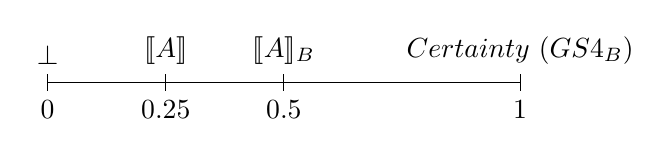
\begin{tikzpicture}
			\begin{centering}
				
				% draw horizontal line   
				\draw (2,0) -- (8,0);
				
				% draw vertical lines
				\foreach \x in {2, 3.5, 5, 8}
				\draw (\x cm,3pt) -- (\x cm,-3pt);
				
				% draw nodes
				\draw (2,0) node[below=3pt] {$ 0 $} node[above=3pt] {$\perp$};
				\draw (3.5,0) node[below=3pt] {$ 0.25 $} node[above=3pt] {\textit{$\llbracket A \rrbracket$}};
				\draw (5,0) node[below=3pt] {$ 0.5 $} node[above=3pt] {$\llbracket A \rrbracket_B$};
				\draw (8,0) node[below=3pt] {$ 1 $} node[above=3pt] {$Certainty$ $(GS4_B)$};
			\end{centering}
			
		\end{tikzpicture}
		
	\end{centering}
	\caption{The values of $\llbracket A \rrbracket$ and $\llbracket A \rrbracket_B$.}
	\label{fig:valuesq}
\end{figure}


It is worth noting that if this sequent was considered in classical logic, it would have different values changing by the value of the atomic formulas, but it would assume value 0 or 1. Something similar happens in Makinson pivotal assumption consequence, also if the belief set is the same that we have defined earlier, because a two valued logic is there considered. 

%The sequent $A$ would have value 0 in classical logic as well as in supraclassical logic with background assumption because at least one of the members has value 0.


\subsection{Strong cut elimination} 

\label{sec:importance_of_cut}

The last section pointed out that the agent is an ideal one and that they are aware of every deduction between beliefs. This means that the belief set is deductively closed: nothing that was not already in the set can be derived.  In order to have a deductively closed belief set it is important that every combination of sentences, when it is possible, must be closed under cut and the new sentences obtained in this way will be added to the belief set. 

In order to eliminate cut from $GS4_B$ the method is taken from \cite{piazzapulcini_uniqueness}, but it is simplified because of the nature of one-sided sequents. The method is the following:

\begin{enumerate}
\item turn each new belief $b_i$ added to the system in a conjunctive form: cnf$(b_i) = b_1 \wedge \dots \wedge b_n$ and add to the system each of the atomic formulas;
\item for each disjunctive formula,  let's remove the application of $\vee$-rule: $b_1 \vee \dots \vee b_n \equiv b_1, \dots , b_n$;
\item let's remove copies of the same sequent;
\item let's remove identity sequents of the form $\vdash \Gamma, p, \overline{p}$;
\item let's close under cut the belief set and add to the system the  new formulas obtained in this way.
\end{enumerate}

It is easy to show why the last step is so important.  Suppose that an agent has a new belief: $A =   (\overline{p} \wedge (\overline{t} \vee q))\vee (t\wedge (\overline{t}\vee q))$. The first thing to do in order to add that belief is to transform $A$ in a conjunctive form: it is easy to show that it is equivalent to $\vdash (\overline{p} \vee t)\wedge(\overline{t}\vee q)\wedge (t \vee \overline{t}\vee q) \wedge (\overline{t} \vee q)$.  Let's decompose it in a set of clauses: $\vdash \overline{p}, t$, $\vdash \overline{t}, q$, $\vdash t, \overline{t}, q$, $\vdash \overline{t}, q$ and remove one of the copies of $\vdash \overline{t}, q$ and the axiom $\vdash t, \overline{t}, q$.  By the method presented earlier the agent has to add $(\overline{p} \vee t)$ and $(\overline{t} \vee q)$ to the system, but these beliefs are not cut free. To let them be cut free, it is necessary to close them under the cut.

	\begin{prooftree}
	\AxiomC{$\vdash \overline{p}, t$}
	
	\AxiomC{$\vdash \overline{t}, q$}
	
	\RightLabel{\scriptsize$(cut)$}
	
	\BinaryInfC{$\vdash  \overline{p}, q$}
\end{prooftree}
\noindent
	From the last point of the method presented earlier, it is needed to add not only $\vdash \overline{p}, t$ and $\vdash \overline{t}, q$, but also $\vdash  \overline{p}, q$. Let's see why:
	$\llbracket (\overline{p} \vee t) \wedge (\overline{t} \vee q) \rrbracket$ has value 1 if $B = \lbrace (\overline{p}, t); (\overline{t}, q)\rbrace$
		

            
            \begin{prooftree}
			\AxiomC{$\sststile{\mathrm{1}}{1}_B \overline{p}, t$}
			\RightLabel{\scriptsize$(\vee)$}
			\UnaryInfC{$\sststile{\mathrm{1}}{1}_B \overline{p} \vee t$}
			
			\AxiomC{$\sststile{\mathrm{1}}{1}_B \overline{t}, q$}
			\RightLabel{\scriptsize$(\vee)$}
			\UnaryInfC{$\sststile{\mathrm{1}}{1}_B \overline{t} \vee q$}
			
			\RightLabel{\scriptsize$(\wedge)$}
			
			\BinaryInfC{$\sststile{\mathrm{2}}{2}_B  (\overline{p} \vee t) \wedge (\overline{t} \vee q)$}
			
		\end{prooftree}
	\noindent 
				But what about $(\overline{p} \vee t) \wedge (\overline{t} \vee q) \wedge (\overline{p} \vee q)$? 
				
					\begin{remark}
						\label{remark:equivalent}
				$(\overline{p} \vee t) \wedge (\overline{t} \vee q) \wedge (\overline{p} \vee q)$ is classically equivalent to $(\overline{p} \vee t) \wedge (\overline{t} \vee q)$, this means that they must have the same value because of stability, i.e. $\llbracket (\overline{p} \vee t) \wedge (\overline{t} \vee q) \rrbracket$ = $\llbracket (\overline{p} \vee t) \wedge (\overline{t} \vee q) \wedge (\overline{t} \vee q) \rrbracket$. 
			\end{remark}
		
	%	\begin{proof}[Remark \ref{remark:equivalent}]
		%	$(\overline{p} \vee t) \wedge (\overline{t} \vee q) \wedge (\overline{p} \vee q) \leftrightarrow (\overline{p} \vee t) \wedge (\overline{t} \vee q)$, i.e., $(p \wedge \overline{t}) \vee (t \wedge \overline{q}) \vee (p \wedge \overline{q})$
		%\end{proof}
		
		What happens if $B = \lbrace (\overline{p}, t); (\overline{t}, q)\rbrace$ is considered, instead of $B = \lbrace (\overline{p}, t); (\overline{t}, q), (\overline{p}, q)\rbrace$, obtained by adding also the belief closed under cut?		
			Let's consider the decomposition of $(\overline{p} \vee t) \wedge (\overline{t} \vee q) \wedge (\overline{p} \vee q)$ within the set $B = \lbrace (\overline{p}, t); (\overline{t}, q)\rbrace$.
			
				\begin{prooftree}
				\AxiomC{$\sststile{\mathrm{1}}{1}_B \overline{p}, t$}
				\RightLabel{\scriptsize$(\vee)$}
				\UnaryInfC{$\sststile{\mathrm{1}}{1}_B \overline{p} \vee t$}
				
				\AxiomC{$\sststile{\mathrm{1}}{1}_B \overline{t}, q$}
				\RightLabel{\scriptsize$(\vee)$}
				\UnaryInfC{$\sststile{\mathrm{1}}{1}_B \overline{t} \vee q$}
				
				\RightLabel{\scriptsize$(\wedge)$}
				
				\BinaryInfC{$\sststile{\mathrm{2}}{2}_B  (\overline{p} \vee t) \wedge (\overline{t} \vee q)$}
				
				\AxiomC{$\sststile{\mathrm{1}}{0}_B \overline{p}, q$}
				\RightLabel{\scriptsize$(\vee)$}
				\UnaryInfC{$\sststile{\mathrm{1}}{0}_B \overline{p} \vee q$}
				
				\RightLabel{\scriptsize$(\wedge)$}
				
				\BinaryInfC{$\sststile{\mathrm{3}}{2}_B  (\overline{p} \vee t) \wedge (\overline{t} \vee q) \wedge (\overline{p} \vee q)$}
				
			\end{prooftree}
		\noindent
		This way a different value for the sequent is obtained and it must have the same value of $\vdash (\overline{p} \vee t) \wedge (\overline{t} \vee q)$. 


This means that it is important to pay attention to frame not only the axioms obtained by the decomposition of the sequent, but also every formula closed under cut. In fact if the set $B = \lbrace (\overline{p}, t); (\overline{t}, q), (\overline{p}, q)\rbrace$ is considered, the original value is restored.

	\begin{prooftree}
	\AxiomC{$\sststile{\mathrm{1}}{1}_B \overline{p}, t$}
	\RightLabel{\scriptsize$(\vee)$}
	\UnaryInfC{$\sststile{\mathrm{1}}{1}_B \overline{p} \vee t$}
	
	\AxiomC{$\sststile{\mathrm{1}}{1}_B \overline{t}, q$}
	\RightLabel{\scriptsize$(\vee)$}
	\UnaryInfC{$\sststile{\mathrm{1}}{1}_B \overline{t} \vee q$}
	
	\RightLabel{\scriptsize$(\wedge)$}
	
	\BinaryInfC{$\sststile{\mathrm{2}}{2}_B  (\overline{p} \vee t) \wedge (\overline{t} \vee q)$}
	
	\AxiomC{$\sststile{\mathrm{1}}{1}_B \overline{p}, q$}
	\RightLabel{\scriptsize$(\vee)$}
	\UnaryInfC{$\sststile{\mathrm{1}}{1}_B \overline{p} \vee q$}
	
	\RightLabel{\scriptsize$(\wedge)$}
	
	\BinaryInfC{$\sststile{\mathrm{3}}{3}_B  (\overline{p} \vee t) \wedge (\overline{t} \vee q) \wedge (\overline{p} \vee q)$}
	
\end{prooftree}
\noindent
Thus the sequents have the same value:

$$\llbracket (\overline{p} \vee t) \wedge (\overline{t} \vee q) \rrbracket_B = \llbracket (\overline{p} \vee t) \wedge (\overline{t} \vee q) \wedge (\overline{p} \vee q) \rrbracket_B = 1$$

As it was showed, the cut is really important for a complete set of beliefs, but it is also necessary to see how the cut can be eliminated from the calculus. 

\paragraph{Elimination of cut}

The elimination of cut in presence of proper axioms was firstly proposed by Girard \cite{gir:prooftypes}, as noted by Avron \cite{avron:gentzen}, upgrading the Gentzen's standard cut elimination algorithm. The procedure here proposed, i.e., the decomposition of the formula, the add to the system and the cut of the formula to obtain all the derivations, owes a lot to the one presented in  \cite{piazzapulcini_uniqueness}. In the article, in fact, is proved that, for any cluster of extra-logical assumptions, there exists exactly one axiomatic extension of classical propositional logic that admits cut elimination.  First of all it is possible to see that weakening it is admissible in $GS4_B$.


\begin{theorem}[Weakening admissibility in $GS4_B$]
	\label{th:weakening}
	For any two atomic formulas $\vdash_B \Gamma$ and $\vdash_B \Delta$, $\llbracket \bigvee \Gamma \vee \bigvee \Delta \rrbracket_B \geq \llbracket \bigvee\Gamma \rrbracket_B$.
\end{theorem}

\begin{proof}
	To prove this is sufficient to consider a transformation of $\vdash _B$. In fact if $B = b_1, \dots b_n$, then $\vdash_B \Gamma$ is equal to $\vdash \Gamma , \overline{b_1}, \dots \overline{b_n}$ with the classical closure as pointed out in \cite{mak:bridges}\footnote{In the text the two sided version of this transformation was used, so $\vdash_B \Gamma$ becomes $b_1, \dots,  b_n \vdash \Gamma$, but here because of the choice to use $GS4$ as main system, it is used the one-sided classically equivalent version $\vdash \Gamma, \overline{b_1}, \dots , \overline{b_n}$.}. Intuitively this is due to the fact that the sequent is true iff there is a disjunction between a letter and its negation (for example $b_i$ and $\overline{b_i}$). From this fact it is possible to consider four cases: 
	
	\begin{itemize}
		\item if $\llbracket \Gamma \rrbracket_B = \llbracket \Delta \rrbracket_B = 1$, than obviously $\llbracket \Gamma \vee \Delta \rrbracket_B = 1$ as well;
		\item if $\llbracket \Gamma \rrbracket_B = \llbracket \Gamma, \overline{b_1}, \dots , \overline{b_n} \rrbracket = 1$ and $\llbracket \Delta \rrbracket_B = 0$, then $\llbracket \Gamma \vee \Delta\rrbracket_B = 1$ as well;
		\item  if $\llbracket \Delta \rrbracket_B = \llbracket \Delta, \overline{b_1}, \dots , \overline{b_n} \rrbracket = 1$ and $\llbracket \Gamma \rrbracket_B = 0$, then  $\llbracket \Gamma \vee \Delta\rrbracket_B \geq \llbracket \Gamma \rrbracket_B$, whatever value assumes  $\llbracket \Gamma \rrbracket_B$;
		\item if $\llbracket \Gamma \rrbracket_B = \llbracket \Delta \rrbracket_B = 0$, then $\llbracket \Gamma \vee \Delta\rrbracket_B \geq \llbracket \Gamma \rrbracket_B$.
	\end{itemize}
\end{proof}

\noindent
It is possible to generalize this result for any context:

\begin{theorem}
	For any context $\Gamma$ and a formula $A$, such that $A$ is not contradictory with the set $B$, $\llbracket \bigvee \Gamma \vee A \rrbracket_B \geq \llbracket \Gamma \rrbracket_B$.
\end{theorem}

\begin{proof}
	Let's prove it by induction on the complexity of the formula $A$.
	
	\begin{description}
		\item[Base case:] Let's consider $A$ atomic, then we have two cases:
		\begin{description}
			\item[$A \in B$:] if $A\in B$, then $\llbracket \bigvee \Gamma, A \rrbracket_B = 1$ and $\llbracket \Gamma, A \rrbracket_B \geq \llbracket \Gamma \rrbracket_B$
			\item[$A \not \in B$:] if $A\not \in B$, then if $\llbracket \bigvee \Gamma \rrbracket_B = 1$, there is an atomic formula in $\Gamma$ that is in the belief set, so also $\llbracket \bigvee \Gamma, A \rrbracket_B = 1$. If $\llbracket \bigvee \Gamma \rrbracket_B = 0$, $b_1 , \dots , b_n \not \in \Gamma$ and then $\llbracket \bigvee \Gamma \vee A \rrbracket_B = 0$
		\end{description}
		\item[Inductive step:] Let's consider two cases:
		\begin{description}
			\item[$A\equiv p\wedge q$:] by inductive hypothesis $\llbracket \bigvee \Gamma \vee p \rrbracket_B \geq \llbracket \Gamma \rrbracket_B$ and $\llbracket \bigvee \Gamma \vee q \rrbracket_B \geq \llbracket \Gamma \rrbracket_B$. If at least one between $\llbracket \bigvee \Gamma \vee p \rrbracket_B$ and $\llbracket \bigvee \Gamma \vee q \rrbracket_B$ is equal to $0$, then $\llbracket \bigvee \Gamma \rrbracket_B = 0$ for inductive hypothesis and then $\llbracket \bigvee \Gamma \vee (p\wedge q) \rrbracket_B \geq \llbracket \Gamma \rrbracket_B$. The only remaining case is when $\llbracket \bigvee \Gamma \vee p \rrbracket_B = 1$ and $\llbracket \bigvee \Gamma \vee q \rrbracket_B =1$:			
			\begin{prooftree}
				\AxiomC{ }
				\UnaryInfC{$\sststile{\mathrm{1}}{1}_B \Gamma, p$}
	\RightLabel{\scriptsize$(\vee)$}
				\UnaryInfC{$\sststile{\mathrm{1}}{1}_B \bigvee \Gamma \vee p$}
			   \AxiomC{ }
			   	\UnaryInfC{$\sststile{\mathrm{1}}{1}_B \Gamma, q$}
	\RightLabel{\scriptsize$(\vee)$}
				\UnaryInfC{$\sststile{\mathrm{1}}{1}_B \bigvee \Gamma \vee q$}
	\RightLabel{\scriptsize$(\wedge)$}
				\BinaryInfC{$\sststile{\mathrm{2}}{2}_B \bigvee \Gamma \vee (p \wedge q)$}
			\end{prooftree}
	\noindent 
			Thus $\llbracket \bigvee \Gamma \vee (p\wedge q) \rrbracket_B \geq \llbracket \Gamma \rrbracket_B$.
			
			\item[$A \equiv p\vee q$:] by theorem \ref{th:weakening}.
		\end{description}
		
		
	\end{description}
\end{proof}

The proof shows that this system is totally monotonic, also if it could seem counterintuitive for a set of belief., because maybe if an agent has a belief $p$ it is strange to believe also $p\wedge q$, but this is due to the fact that this work is based on a classical framework and so the fractional value of $\llbracket p \rrbracket_B$ assumes the same of $\llbracket p\wedge q \rrbracket_B$.

\begin{theorem}[Strong cut elimination of $GS4_B$]
	\label{th:cut_elimination_GS4_B}
	The cut rule is redundant when added to $GS4_B$.
\end{theorem}

\begin{proof}
	Recalling that it is possible to push upwards the application of cut rule, it is possible to reduce the cut to:
	
	\begin{prooftree}
		\AxiomC{$\vdots$}
		\noLine
		
		\UnaryInfC{$\vdash_B \Delta , p$}
		
		\AxiomC{ }
					\RightLabel{\scriptsize$(b_i)$}
				\UnaryInfC{$\vdash_B \Delta , \overline{p}$}
				\RightLabel{\scriptsize$(cut)$}
			\BinaryInfC{$\vdash_B \Delta$}
	\end{prooftree}

	With this formulation is not possible to see the proper axioms added to the system, thus as before it is possible to transform them into a disjunction of the negation of each belief in $\vdash \Delta, p, \overline{b_1}, \dots \overline{b_n}$ and $\vdash \Delta, \overline{p}, \overline{b_1}, \dots \overline{b_n}$ as done before. The new version of cut will be:
	
		\begin{prooftree}
		\AxiomC{$\vdots$}
		\noLine
		\UnaryInfC{$\vdash \Delta, p, \overline{b_1}, \dots, \overline{b_n}$}
		
		\AxiomC{ }
				\RightLabel{\scriptsize$(b_i)$}
		\UnaryInfC{$\vdash \Delta, \overline{p}, \overline{b_1},  \dots, \overline{b_n}$}
		\RightLabel{\scriptsize$(cut)$}
		\BinaryInfC{$\vdash \Delta,\overline{b_1},  \dots, \overline{b_n}$}
	\end{prooftree}

Because of the fact that $\vdash_B \Delta , \overline{p}$ is introduced by a belief, i.e., the value is 1, and it has no occurrences of $\wedge$, then or one of the formula in the multiset $\Delta$ is in $B$, or $\overline{p} \in B$. If $\overline{p} \in B$ then one of the negation of beliefs, will be $p$. This means that $\vdash \Delta,  p, \overline{b_1},\dots , \overline{b_n}$ is equivalent to $\vdash \Delta, \overline{b_1},\dots , \overline{b_n}$.
\noindent
On the other hand:


	\begin{prooftree}
	\AxiomC{$\vdots$}
	\noLine
	\UnaryInfC{$\vdash \Delta, p, \overline{b_1}, \dots, \overline{b_n}$}
	
	\AxiomC{ }
	\RightLabel{\scriptsize$(b_i)$}
	\UnaryInfC{$\vdash \Delta, \overline{p}, \overline{b_1},  \dots, \overline{b_n}$}
	\RightLabel{\scriptsize$(cut)$}
	\BinaryInfC{$\vdash \Delta,\overline{b_1},  \dots, \overline{b_n}$}
\end{prooftree}

\noindent
becomes directly the introduction of the belief:

\begin{prooftree}
		\AxiomC{ }
	\RightLabel{\scriptsize$(b_i)$}
 \UnaryInfC{$\vdash \Delta, \overline{b_1},\dots , \overline{b_n}$}
\end{prooftree}



\end{proof}

The set of beliefs can be ``completed'' through cut or without that. This means that $GS4_B$ is a cut-free system, because it is an axiomatic extension of classical logic. By the way, the use of cut can alter the fractional semantics value as shown in \cite{piazzapulcini:fractional}. Thanks to theorem \ref{th:cut_elimination_GS4_B} the algorithm presented in section \ref{sec:importance_of_cut} can be transformed in an algorithm without the presence of cut. As a corollary of the strong cut elimination it can be obtained:


\begin{theorem}[Uniqueness of axiomatization in $GS4_B$]
	For any cluster of axioms in the set of beliefs $B$ the axiomatization is unique.
\end{theorem}

\begin{proof}
	See \cite{piazzapulcini_uniqueness}.
\end{proof}


\section{Fractional semantics, Lockean Thesis and the paradox of Lottery}

An interesting application of the fractional semantics for classical logic can be found in the solution of a traditional problem: the lottery paradox. The lottery paradox is deeply related to the Lockean Thesis: a way to define how classical logic coheres with  beliefs. 
 
Briefly speaking, the Lockean Thesis states that an agent can choose a rational number in the interval [0,1] for the semantic interpretation of a formula that works as a truthfulness threshold and imposes after which number an agent considers true a certain proposition or a set of propositions. Thus, for instance, an agent assigns to the threshold the value of 0.9 if the sentence considered has a value greater than 0.9, then the sentence will be considered as true as a tautology, otherwise it will be considered as false. The name of ``Lockean thesis'' is  not given because Locke itself proposed it, but because in  ``An essay concerning human understanding'', talking about the probability writes:

\begin{quote}
	<<But another Man who never took the pains to observe the Demonstration, hearing a Mathematician, a Man of credit, affirm the three Angles of a Triangle, to be equal to two right ones, assents to it: i.e. receives it for true.>>\footnote{John Locke, \textit{An essay concerning human understanding} (1690) $4^{th}$ book, chapter XV, \S1}
\end{quote}

The beliefs are related to the level of assent that one agent can give to another and so to those beliefs that are not 100\% true, but in which the agent still has a high degree of confidence in them. 

\begin{quote}
	<<Being that which [the probability] makes us presume things to be true, before we know them to be so.>>\footnote{ivi. $4^{th}$ book, chapter XV, \S 3}
\end{quote}

Here probability is treated as the level of assent in a certain proposition, in fact the renewed version of the Lockean Thesis is formulated as it follows in \cite{Foley_epistemology}: 

\begin{quotation}
	\emph{It is epistemically rational for us to believe a proposition just in case it is epistemically rational for us to have a sufficiently high degree of confidence in it, sufficiently high to make our attitude towards it one of belief.}
\end{quotation}

The Lockean thesis has a lot of important positive aspects, for example it implies that even a logically ideal agent whose degrees of confidence satisfy the axioms of probability theory, may quite rationally believe each of a large body of propositions that are jointly inconsistent. For the Lockean Thesis, in fact, as we will properly see, the beliefs are not closed under conjunction, because it is possible to have inconsistent beliefs with different degree of confidence in them. On the other hand the Lockean thesis does not clarify how to choose the threshold and sometimes it seems a little rough-edged. By the way the main problem of the Lockean Thesis is made by the \textit{Lottery Paradox}, a paradox easy at first sight, but that come into conflict with the Lockean Thesis. 

\paragraph{The Lottery Paradox}
	
	Suppose a fair 1000-ticket lottery that has exactly one winning ticket. A perfectly rational agent knows that one ticket has the probability of 999/1000 to be a not winning ticket. This means that is rational to accept that one ticket will not win because is greater than every rational Lockean threshold. This procedure can be applied also to every other ticket in the lottery and this means that somehow every ticket will not be a winning ticket, but the lottery is fair, so the conjunction between all these sentences has to be true and not false as it appears. 

	This apparently easy paradox points out a very interesting problem. The problem can be formalized in modal logic through the Barcan formula (BF). While the converse Barcan formula (CBF) is not problematic, the Barcan formula is problematic when considered with the lottery paradox.
	
	\begin{equation}
		\tag{BF}
		\forall x \Box F(x) \rightarrow \Box \forall x F(x)
	\end{equation}
\begin{equation}
	\tag{CBF}
	\Box \forall x F(x) \rightarrow \forall x \Box F(x)
\end{equation}

The converse Barcan formula is not problematic in this case, because points out that if it is necessary that all $x$ has the property $F$, than each $x$ must have the property $F$. This means that if it is necessary that every ticket is a losing one, than for all tickets, each one will be a losing one. 

On the other hand the Barcan formula points out that if every x is necessarily $F$, then it is necessary that every $x$ is $F$ or, in the considered case, if it is necessary that for all tickets, each ticket considered alone will be a losing one, then it is necessary that every ticket is a losing ticket. This is problematic because if the Lockean Thesis and the threshold are considered, then each ticket considered alone will be a losing ticket, but also the conjunction of all the losing ticket will be considered true, that is obviously false.

	
	One of the solutions to this problem (for example in \cite{Hawthorne2009-HAWTLT} and \cite{Leitgeb_stability}) is to affirm that beliefs are not closed under conjunction, but this is a very strong  thesis. The reason why beliefs can't be closed under a conjunction, in the authors' opinion, is related to the fact that beliefs are not totally certain, they can change value or maybe themselves, and for this reason it is possible to have more than one inconsistent beliefs at once.

	By the way, it could be useful to close beliefs under conjunction and, considering the Lockean Thesis, this is not possible even for consistent sets. Through Fractional Semantics it is easy to establish a way that saves classical logic and the conjunction between beliefs.

	Let's call the sentence ``The ticket $n$ will win'' as $p_n (1\leq n \leq 1000)$ and let's call the only winning ticket $p_i$. With a little lack of generalization (in this case the first and the last ticket couldn't be a winning ticket) it is possible to enumerate the tickets in this way: $p_1, \dots, p_{i-1}, p_i, p_{i+1}, \dots, p_{1000}$. To write the problem better it is possible to consider the negations, i.e., $\overline{p_1}, \dots,  \overline{p_i}$ and put them into a tree. The fractional semantics value of a single not winning ticket will be true and it will be false only for the winning ticket. The tree works in the same way also if the first or the last ticket is a winning one.
	
	\begin{prooftree}
		
\AxiomC{ }
\RightLabel{\scriptsize }
\UnaryInfC{$\sststile{\mathrm{1}}{1}_{B} \overline{p_1}$}
	
	\AxiomC{$\dots$}

	\AxiomC{ }
	\RightLabel{\scriptsize }
	\UnaryInfC{$\sststile{\mathrm{1}}{1}_{B} \overline{p_{i-1}}$}

	\TrinaryInfC{$\sststile{\mathrm{i-1}}{\mathrm{i-1}}_{B} \overline{p_1} \wedge \dots \wedge \overline{p_{i-1}}$}
	
		\AxiomC{ }
	\RightLabel{\scriptsize }
	\UnaryInfC{$\sststile{\mathrm{1}}{0}_{B} \overline{p_{i}}$}
	
	\BinaryInfC{$\sststile{\mathrm{i}}{\mathrm{i-1}}_{B} \overline{p_1} \wedge \dots \wedge \overline{p_{i-1}} \wedge  \overline{p_{i}}$}
	
		\AxiomC{ }
	\RightLabel{\scriptsize }
	\UnaryInfC{$\sststile{\mathrm{1}}{1}_{B} \overline{p_{i+1}}$}
	
	\BinaryInfC{$\sststile{\mathrm{i+1}}{\mathrm{i}}_{B} \overline{p_1} \wedge \dots \wedge \overline{p_{i-1}} \wedge  \overline{p_{i}} \wedge \overline{p_{i+1}}$}
	
		\AxiomC{$\dots$}
		
				\AxiomC{ }
		\RightLabel{\scriptsize }
		\UnaryInfC{$\sststile{\mathrm{1}}{1}_{B} \overline{p_{1000}}$}
	\TrinaryInfC{\vdots}
	\UnaryInfC{$\sststile{\mathrm{1000}}{999}_{B} \overline{p_1} \wedge \dots \wedge \overline{p_{i-1}} \wedge  \overline{p_{i}} \wedge \overline{p_{i+1}} \wedge \dots \wedge \overline{p_{1000}}$}
	
\end{prooftree}
\noindent 



Fractional semantics deals perfectly with this paradox, providing a very simple solution to this problem. In fact it is easy to see that in fractional semantics it is not useful to have a threshold, because in every moment is possible to control the value of a proposition and also the history of how that value becomes itself thanks to the proof tree. 
The final value will be 999/1000 and means that 999 parts of the conjunction are true out of the 1000 joints and this coheres with the fact that one ticket must be the winning one.  

\paragraph{Fractional semantics and probability}
Must be stressed here that the fractional semantics value is not a probabilistic one, in fact the probability measure of the conjunction is made by the conditionalization formula as pointed out in \cite{halpern:reasoning}. In this formalism $\mathcal{P}$ indicates the probability,  $\mathcal{P}(\overline{p_1})|\mathcal{P}(\overline{p_2})$ indicates the probability that the event $\overline{p_2}$  happens once $\overline{p_1}$ happened. This is called conditionalization because it is the probability that a certain event happens if another happened, conditiong the final probability and it is calculated by the following formula.


$$\mathcal{P}(\overline{p_1} \wedge \overline{p_2}) = \mathcal{P} (\overline{p_1})\cdot (\mathcal{P} (\overline{p_1})|\mathcal{P}(\overline{p_2}))$$

\noindent
This means that, once $\overline{p_1}$ is realized, also $\overline{p_2}$ realizes, so:

$$\mathcal{P}(\overline{p_1} \wedge \overline{p_2}) = \frac{999}{1000} 	\cdot \frac{998}{999} = \frac{998}{1000}$$

%This is also intuitive by the fact that if the probability of $p_1$ is 1/1000, the probability of the conjunction $p_1 \wedge p_2$ will be 2/1000. 

The meaning of the fractional semantics value is that the conjunction is true for 999 of the joints and false for only one of them. Where the probability or classical logic assigns value 0, fractional semantics helps us to understand that, also if the final conjunction results false in classical logic, actually all but one of the propositions are true and this result is not explicit in classical framework.


\section{Conclusions}

The present research may be considered as an attempt to create a bridge between logic and the real world, nonetheless retaining consistency and decidability.

The main difference between classical approach and the fractional semantics one is either philosophical and technical. By a technical point of view is possible to distinguish between different levels of contradiction. Fractional semantics is able to distinguish between what's inside truthfulness and falsity, without losing the rigorous approach to proof theory, proving the cut elimination and the others fundamental properties. 

The system $GS4_B$ is able to consider beliefs and logical axioms together. The fractional system, in fact, does not have the symmetry between tautologies and contradictions and it is helpful to talk about something that is uncertain such as beliefs. We have shown that fractional semantics could be useful to see how to solve a simple, but tricky problem such as the Lottery Paradox. 

It's interesting to see how fractional semantics behaves differently compared to classical interpretation and probability. It was important to point out the difference between probability and fractional semantics, also because it will not be strange that fractional semantics and probability will be able to work together to better define logical derivations involving beliefs. 



\paragraph{Further researches} This kind of implementation could be expanded even more, for example considering restrictions of the set of beliefs,i.e., applying fractional semantics to non monotonic logics or non classical logics in general.

In the Paradox of lottery it was interesting to notice that these different results, interpreted together, can be richer in content than probability itself, letting know, through a value, the number of true and false conjuncts propositions. Despite this, a way to let probability, fractional semantics and maybe belief revision work together must be implemented yet.

 \addcontentsline{toc}{section}{\refname}
\nocite{*}

\printbibliography
\end{document}
